\documentclass[a4paper,10pt,titlepage]{article} \usepackage[utf8]{inputenc}
\usepackage{a4wide} \usepackage[czech]{babel}
\usepackage[small,compact]{titlesec}

\usepackage{graphicx}
\usepackage{amsthm}
\usepackage{amsmath}
\usepackage{amsfonts}
\usepackage{amssymb}

\newtheorem{theorem}{Věta}
\newtheorem{define}{Definice}
\newtheorem*{notation}{Značení}
\newtheorem*{example}{Příklad}
\newtheorem*{remark}{Poznámka}

\begin{document} \pagestyle{empty}
\begin{center}
\textbf{zaměření Diskrétní modely a struktury}

\textit{by Veronika Slívová, veronika.slivova@gmail.com}
\end{center}
\medskip

{\sc{požadavky}}

\begin{enumerate}
\item Množiny a zobrazení
\item Subvalence a ekvivalence množin
\item Dobré uspořádání
\item Axiom výběru (Zermelova věta, Zornovo lemma)
\item Barvení grafu (Brooksova a Vizingova věta)
\item Tutteova věta
\item Extremální kombinatorika (Ramseovy věty, Erd\H{o}s-Ko-Radoova věta)
\item Samoopravné kódy
\item Pravděpodobnostní metoda - příklady použití
\end{enumerate}


\medskip

\section{Množiny a zobrazení}

Výskyt proměnné $x$ je \textit{vázaný} pokud je součástí podformule $(\forall x) \varphi(x)$ nebo $(\exists x) \varphi(x)$.
Jinak je výskyt proměnné \textit{volný}. 
Proměnná je \textit{vázaná} v nějaké formuli, má-li v ní vázaný výskyt.
Naopak proměnná je \textit{volná} v nějaké fli, má-li v ní volný výskyt.

\subsection{Axiomy teorie množin}

\begin{enumerate}
\item {\sc{axiom existence}} - ``existuje množina''
\[
	(\exists x) (x=x)
\]
\item {\sc{axiom extensionality}} - ``množiny, obsahující tytéž prvky jsou si rovny''
\[
	(\forall u) (u\in x \Leftrightarrow u \in y) \implies (x=y)
\]
\item {\sc{schéma axiomů vydělení}} - ``z každé množiny lze vydělit množinu prvků splňujících nějakou formuli''

Fle $\psi$ neobsahuje volnou proměnou $z$.
\[
	(\forall a) (\exists z) (\forall x) ((x\in z) \Leftrightarrow (x \in a \wedge \varphi(x)))
\]
\item {\sc{axiom dvojice}} - ``libovolné dvě množiny určují dvouprvkouvou množinu''
\[
	(\forall a) (\forall b) (\exists z) (\forall x) ((x \in z) \Leftrightarrow (x=a) \vee (x=b))
\]
\item {\sc{axiom sumy}} - ``ke každé množině existuje množina sestávající ze všech prvků jejích prvků''
\[
	(\forall a) (\exists z) (\forall x) ((x \in z) \Leftrightarrow (\exists y) ((y \in a) \wedge (x \in y)))
\]
\item {\sc{axiom potence}} - ``Ke každé množině existuje množina všech jejích podmnožin''
\[
	(\forall a) (\exists z) (\forall x) ((x \in z) \Leftrightarrow (x \subseteq a))
\]
\item {\sc{schéma axiomů nahrazení}} - ``Definovatelné zobrazení zobrazuje množinu na množinu''

Formule $\psi$ neobsahuje volně proměnné $w$ a $z$
\[
	(\forall u) (\forall v) (\forall w) ((\psi(u,v) \wedge \psi(u,w)) \Rightarrow (v=w)) \implies
	(\forall a) (\exists z) (\forall v) ((v\in z) \Leftrightarrow (\exists u) ((u \in a) \wedge \psi(u,v)))
\]
\item {\sc{axiom nekonečna}} - ``Existuje nekonečná množina''
\[
	(\exists z) ((0 \in z) \wedge (\forall x) ((x \in z) \Rightarrow (x \cup \{x\} \in z)))
\]
\item {\sc{axiom fundovanosti (regularity)}}
\[
	(\forall a) (a \neq 0 \Rightarrow \exists x ((x \in a) \wedge (x \cap a = 0)))
\]
\end{enumerate}

{\sc{Poznámky k axiomům}}
\begin{itemize}
\item Schéma axiomů nahrazení a schéma axiomů vydělení, jedná se o nekonečně mnoho axiomů, pro každou fli jeden axiom.

\item Symboly $\subseteq,\ 0,\ \cup,\ \cap,\ \{x\}$ nejsou v základním jazyce teorie množin, jedná se o zkratky

\item (add Schéma axiomů vydělení) $z$ nesmí být volně ve $\phi$ protože po dosazení fle $\phi(x) = x \notin z$ je axiom sporný.
		(Podobně i u schéma axiomů nahrazení zakazujeme volné výskyty $w$ a $z$)
\end{itemize}

\begin{define}
(Relace)

Binární relace je množina $r$ jejímiž prvky jsou uspořádané dvojice
\end{define}

\begin{define}
(Definiční obor, Obor hodnot)

Pro relaci $r$ definujeme definiční obor $D_f = \{x: (\exists y) <x,y> \in r \}$
a obdobně obor hodnot \\ $H_f = \{y: (\exists x) <x,y> \in r \}$.
\end{define}

\begin{define}
(Inverzní relace)

Pro relaci $r$ definujeme inverzní relaci $r^{-1} = \{\langle y , x \rangle  | \langle x , y \rangle  \in r\}$.
\end{define}

\begin{define}
(Složení relací)

Pro relace $r,s$ definujeme jejich složení $r\circ s = \{\langle x , z \rangle  | \langle x , y \rangle  \in r\ \wedge\ \langle y , z \rangle  \in s\}$.
\end{define}

\begin{define}
(Funkce)

Relaci $f$ nazveme funkce pokud platí následující
\[
	(\forall x \in D_f(f)) ((y\in H_f(f)) \ \wedge \ (y'\in H_f(f)) \ \wedge \ (\langle x , y \rangle  \in f)
	\ \wedge \ (<x,y'> \in f)) \implies (y=y')
\]
\end{define}

\begin{define}
(Zúžené zobrazení)

Je-li $f: a\rightarrow b$ funkce a $c\subseteq a$, pak $f \upharpoonright c = f \cap (c\times b)$ se nazývá zúžením 
funkce $f$ na množinu~$c$.
\end{define}

\begin{define}
(Prostá, Surjektivní, Bijekce)

Funkce $f: a\rightarrow b$ je 
\begin{enumerate}
\item prostá - je-li $f^{-1}$ funkce,
\item surjektivní (na) - je-li $H_f(f) = b$,
\item bijekce - je-li prostá i na.
\end{enumerate}
\end{define}

\begin{define}
(Podmnožina, vlastní podmnožina)

Množina $x$ je podmnožinou $y$ ($x\subseteq y$), pokud platí $(\forall t) (t \in x) \Rightarrow (t \in y)$.

Množina $x$ je vlastní podmnožinou $y$ ($x\subset y$), pokud $x\subseteq y \wedge x \neq y$
\end{define}

Z axiomů se dají dokázat následující vlastnosti:
\begin{enumerate}
\item $x\subseteq x$, $\neg(x \subset x)$
\item $(x \subseteq y \wedge y \subseteq z) \Rightarrow x \subseteq z$
\item $(x \subset y \wedge y \subset z) \Rightarrow x \subset z$

	  $(x \subseteq y \wedge y \subset z) \Rightarrow x \subset z$
	
	  $(x \subset y \wedge y \subseteq z) \Rightarrow x \subset z$
\item $(x \subseteq y \wedge y \subseteq x) \Rightarrow x = y$
\end{enumerate}

\section{Dobré uspořádání}
\begin{define}
(Ostře uspořádaná množina)

Ostře uspořádaná množina je uspořádaná dvojice $\langle a , r \rangle $, kde $a$ je množina a $r\subseteq a \times a$ je relace splňující:
\[
((\langle x , y \rangle  \in r)\ \wedge\ (\langle y , z \rangle  \in r)) \Rightarrow \ \langle x , z \rangle  \in r
\]
\[
(\forall x \in a)\ \neg (\langle x , x \rangle  \in r)
\]
\end{define}

\begin{notation}
U uspořádaní používáme značení $(x\ r\ y)$ místo $(x,y) \in r$.
\end{notation}

\begin{define}
(Lineární uspořádání)

Ostré uspořádání je lineární, jestliže
\[
 (\forall x,y \in a)\ ((x=y) \vee (x\ r\ y) \vee (y\ r\ x))
\]
\end{define}

\begin{define}
(Nejmenší prvek)

Je-li $r$ uspořádání na množině $a$, $m \subseteq a$, $x \in a$, pak $x$ je nejmenší prvek množiny $m$
pokud $x \in m$ a zároveň $(\forall y \in m)\ ((x = y)\ \vee \ (x\ r\ y))$.
\end{define}

\begin{define}
(Dobré uspořádání)

Uspořádání $r$ je na množině $m$ dobré ($m$ je dobře uspořádaná množina relací $r$), pokud každá neprázdná podmnožina $m$ má nejmenší prvek.
\end{define}

\begin{example}
$\mathbb{R}$ s relací $<$ je dobře uspořádaná množina

$\{\frac{1}{n}\ |\ n \in \mathbb{Z}^+\}$ a $<$ není dobře uspořádaná množina

$ \{0\} \cup \{\frac{1}{n}\ |\ n \in \mathbb{Z}^+\}$ a $<$ také není dobře uspořádaná množina.

$\{1-\frac{1}{n}\ |\ n \in \mathbb{Z}^+\}$ je dobře uspořádaná množina
\end{example}

\begin{define}
(Izomorfismus uspořádaných množin)

Jsou-li $a,b$ množiny, $r,s$ relace, pak $< a,r >$ je isomorfní $< b,s >$ pokud existuje bijekce $f: a \rightarrow b$ taková, že
\[
(x\ r\ y) \Leftrightarrow (f(x)\ s\ f(y))
\]
Zobrazení $f$ nazýváme izomorfismus.
\end{define}

\begin{define}
(Počáteční úsek)

Počáteční úsek množiny $\langle a , r \rangle $ je podmnožina $\{ y\ |\ (y \in a) \wedge (y\ r\ x)\}$.
Budeme jej značit $(\leftarrow , x)$.
\end{define}

\begin{theorem}\label{l1}
Je-li $< a,r >$ dobře uspořádaná množina, pak $\forall x \in a$ platí $< a,r >$ není isomorfní s~$< (\leftarrow,x), r>$.
\end{theorem}

\begin{proof}
Dokazuje se sporem. Vezmeme si nějaký izomorfismus $f$.
Nalezneme nejmešní $t$ takové, že $f(t) \neq t$.
Rozdělíme na dva případy $(f(t)\ r\ t)$ pak $f$ není prosté, nebo
$(t\ r\ f(t))$ pak $f$ není surjektivní (na).
\end{proof}

\begin{theorem}\label{l2}
Jsou-li $< a,r >$ a $< b,s >$ dvě dobře uspořádané množiny, pak mezi nimi existuje jedinný izomorfismus.
\end{theorem}

\begin{proof}
Sporem, obdobně jako předchozí věta. Máme dva izomorfismy $f,g$ najdeme nejmenší prvek $y_0$, ve kterém se liší.
Pak pokud $(f(y_0)\ s\ g(y_0))$ pak $g$ není surjektivní. Jinak $(g(y_0)\ s\ f(y_0))$ a $g$ není prostá.
\end{proof}

\begin{theorem}
Jsou-li $< a,r >$ a $< b,s >$ dvě dobře uspořádané množiny, pak nastane jedna z možností:
\begin{enumerate}
\item  $< a,r >$ je izomorfní $< b,s >$ 
\item  $(\exists y \in b)\ < a,r > \ \cong \ < (\leftarrow , y),s >$ 
\item  $(\exists x \in a)\ < (\leftarrow , x),r > \ \cong \ < b,s >$ 
\end{enumerate}
\end{theorem}

\begin{proof}
Položíme 
\[
	f = \{\langle v , w \rangle \ | \ v \in a\ \wedge \ w \in b\ \wedge \ (<(\leftarrow ,v), r> \ \cong \ < (\leftarrow , w),s >)
\]
Postupně ukážeme, že
\begin{enumerate}
\item $f$ je funkce	($\langle v , w \rangle  \in f$ a $<v,w_2> \in f$ pak 
\[
	<(\leftarrow , w), s>\ \cong \ <(\leftarrow , v), r> \ \cong \ <(\leftarrow , w), s>,
\]
což je spor s větou \ref{l1})
\item $f$ je prostá (obdobně jako předchozí)
\item $f$ zachovává uspořádání (díky větě \ref{l2}, protože $f$ je izomorfismus počátečních úseků)
\item prázdnost alespoň jedné z množin
$ m = \{v \in a | (\forall w \in b) \ \langle v , w \rangle  \notin f\}$
a \\$o = \{w \in b | (\forall v \in a) \ \langle v , w \rangle  \notin f\}$
(jsou-li obě neprázdné tvoří $f$ izomorfismus mezi jejich nejmenšími prvky)
\end{enumerate}
\end{proof}


\begin{define}
(Tranzitivní množina)

Množina $x$ je tranzitivní, pokud $\forall y  y \in x \Rightarrow y \subseteq x$. 
\end{define}

\begin{define}
(Ordinál)

Ordinál je dobře uspořádaná tranzitivní množina.
\end{define}

\begin{notation}
Pro ordinály $\alpha, \beta$ budeme psát $\alpha < \beta$ pokud $\alpha \in \beta$ a
$\alpha \leq \beta$ pokud $\alpha < \beta$ nebo $\alpha = \beta$.
\end{notation}

\begin{define}
(Následník)

Pro ordinál $\alpha$ definujeme následníka $s(\alpha ) = \alpha \cup \{\alpha\}$.
\end{define}

\begin{define}
(Isolovaný a limitní ordinál)

Ordinál $\alpha$ nazveme isolovaným pokud $\alpha = 0$ nebo existuje ordinál $\beta$ tž. $\alpha = s(\beta)$.
Jinak je ordinál $\alpha$ limitní.
\end{define}

\begin{define}
(Přirozené číslo)

Ordinál $\alpha$ je přirozené číslo jestliže $(\forall \beta) (\beta \leq \alpha)$ platí $\beta$ je isolovaný ordinál.
\end{define}

\begin{remark}
Množinu všech přirozených čísel získáme z axiomu nekonečna a budeme značit $\omega$.
\end{remark}

\section{Subvalence a ekvivalence množin}
\begin{define}
(Subvalence a ekvivalence množin)
Množina $x$ je subvalentní $y$ neboli mohutnost množiny $x$ je menší rovna mohutnosti množiny $y$,
pokud existuje prosté zobrazení $f: x \rightarrow y$. ($x \preceq y$)

Množina $x$ je ekivalentní $y$ neboli mohutnost množiny $x$ je rovna mohutnosti množiny $y$,
pokud existuje bijekce $f: x \rightarrow y$. ($x \approx y$)

Množina $x$ je ostře subvalentní $y$ neboli mohutnost množiny $x$ je menší rovna mohutnosti množiny $y$,
pokud $x$ je subvalentní $y$ a zároveň $x$ není ekvivalentní $y$.  ($x \prec y$)
\end{define}


\begin{theorem}
(Cantor-Bernsteinova věta)

$x,y$ libovolné dvě množiny, pak platí
\[
(x \preceq y) \ \wedge \ (y \preceq x) \implies (x \approx y)
\]
\end{theorem}

\begin{proof}
Máme zobrazení $f: x \rightarrow y$ a $g: y \rightarrow x$ prostá.
Navíc $H_f(f) \subset y$ a $H_f(g) \subset x$.
Pro všechna přirozená čísla definujeme indukcí $a_0 = a$, $b_0 = b$, $a_n = H_f(f\upharpoonright b_{n-1})$ a
$b_n = H_f(f\upharpoonright a_{n-1})$. Dále definujeme $a_{\omega} = \bigcap \{a_n | n \in \omega\}$ a
$b_{\omega} = \bigcap \{b_n | n \in \omega\}$.

Potom můžeme definovat zobrazení $h: x \rightarrow y$:
\begin{center}
$h(x) = f(x)$  pro $x \in \left(\bigcup_{n \in \omega} a_{2n} \setminus a_{2n+1}) \cup a_{\omega}\right)$

$h(x) = t$  pro $x = g(t)$ a $x \in \left(\bigcup_{n \in \omega} a_{2n+1} \setminus a_{2n}) \cup a_{\omega}\right)$
\end{center}
Ověříme, že $h$ je prostá a surjektivní $\rightarrow$ $h$ je hledaná bijekce.
\end{proof}

\begin{define}
(Mohutnost množiny)

Pro množinu $a$ definujeme její mohutnost $|a|$ jako nejmenší ordinál $\alpha$ takový, že $\alpha \approx a$.
\end{define}

\begin{define}
(Kardinál)

Kardinál je takový ordinál $\alpha$, pro který platí $|\alpha| \approx \alpha$.
\end{define}

\begin{theorem}
(Cantorova věta)

Pro každou množinu $x$ platí $x \prec \mathcal{P}(x)$, kde $\mathcal{P}(x)$ je potenční množina $x$ (viz axiom potence).
\end{theorem}

\begin{proof}
$x \preceq \mathcal{P}(x)$ triviální

Stačí ukázat, že neplatí $x \approx \mathcal{P}(x)$, tedy neexistuje bijekce $f: x \rightarrow \mathcal{P}(x)$.
Nechť $g: x \rightarrow \mathcal{P}(x)$ je libovolné zobrazení.
Pak $g$ nezobrazí žádný prvek na množinu $y = \{t\in x\  |\ t \notin g(t)\}$, tedy $g$ není surjektivní a tedy není bijekce.
\end{proof}

\section {Axiom výběru (Zermelova věta, Zornovo lemma)}

\begin{define}
(Kartézský součin souboru množin)

Nechť $a$ je množina a $< x_t :\ t\in a>$ je soubor množin pak kartézský součin souboru $< x_t :\ t\in a>$ je
\[
	\prod_{t \in a} x_t = \left\{f \left| \ \left(f:a \rightarrow \bigcup_{t \in a} x_t\right) \ 
	\wedge \ \left(\forall t \in a\right) f(t) \in x_t \right. \right\} 
\]
\end{define}

\begin{define}
(Rozklad množiny)

Množina $r$ je rozkladem množiny $x$, pokud $x = \bigcup r$, $0 \notin r$ a $(\forall u,v \in r)((u \neq v) \Rightarrow (u \cap v = 0))$.
\end{define}

\begin{define}
(Selektor)

Selektor $f$ je funkce definovaná na množině $x$, $f: x \rightarrow \bigcup x$ taková, že
\[
	((y \in x) \ \wedge \ (y\neq 0)) \ \implies\ (f(y) \in y).
\]
\end{define}

\medskip
{\sc{Princip výběru}}

Pro každý rozklad $r$ množiny $x$ existuje množina $y$ taková, že
\[
	(\forall u \in r) (\exists t) ( y \cap u = \{t\}).
\]

Množinu $y$ pak nazýváme výběrovou množinou pro rozklad $r$.

\medskip
{\sc{Axiom výběru}}

Na každé množině existuje selektor.

\medskip

\begin{theorem}
Následující tvrzení jsou ekvivalentní
\begin{enumerate}
\item Axiom výběru
\item Princip výběru
\item Pro každou relaci $s$ ecistuje fce $f$ tž. $f \subseteq s$ a $D_f(f) = D_f(s)$
\item Je-li $x$ neprádná a $<y_t : t \in x>$ soubor neprázdných množin pak jeho kartézský součin je neprázdný.
\end{enumerate}
\end{theorem}

\begin{proof}
$((1)\rightarrow(2)):$ $f$ selektor, pak $H_f(f)$ je výběrová množina

$((2)\rightarrow(3)):$ je-li $s$ prázdná je i $f$ prázdná jinak $f$ je výběrová množina pro soubor množin
$\{ \{\langle u , v \rangle | \langle u , v \rangle  \in s\}\ |\ \forall u \in D_f(s) \}$

$((3)\rightarrow(4)):$ definujeme relaci $s = \{\langle t , v \rangle  \ |\ (t\in x) \ \wedge\ (v \in y_t) \}$, dle $(3)$ existuje funkce $f$.
Pak funkce $f$ patří do kartézkého součinu souboru $<y_t : t \in x>$.

$((4)\rightarrow(1)):$ Buď $x$ neprázndná množina neobsahující prázdnou množinu, pak libovolná funkce $f$ z kartézského součinu na souboru $x$
je selektorem na $x$.
\end{proof}

\begin{define}
(Řetězec)

$a$ množina uspořádaná relací $\leq$, pak $c \subseteq a$ je řetězec, je-li uspořádán relací $\leq$ lineárně.
\end{define}

\begin{define}
(Horní mez, Maximální prvek)

Nechť $a$ je množina uspořádaná relací $\leq$ a $b\subseteq a$. 
Prvek $x$ se nazývá horní mezí množiny $b$ pokud $(\forall y \in b)\ y\leq x$.

Prvek $m$ se nazývá maximem množiny $b$ pokud $m \in b \ \wedge \ (\forall y \in b) \ \neg(y > m)$.
\end{define}

\medskip
{\sc{Princip maximality (Zorn-Kuratowského lemma)}}

Nechť $a$ je množina uspořádaná relací $\leq$ taková, že každý řetězec má horní mez.

Pak existuje maximální prvek množiny $a$.

\medskip
{\sc{Princip dobrého uspořádání (Zermelova věta)}}

Pro každou množinu $a$ existuje relace, která je dobrým uspořádáním na $a$.

\medskip

V důkazu následující věty použijeme pojem transfinitní rekurze. 
Jedná se o "funkci" $G$ z ordinálů $O_n$ do třídy všech množin $V$,
takovou, že
\[
	G(\alpha) = F(G \upharpoonright \alpha),
\]
kde $F$ je nějaká "funkce" z $V$ do $V$. (Nejde o funkce protože $V$ a $O_n$ nejsou množiny).
Z věty o transfinitní rekurzi víme, že existuje právě jedna taková "funkce" $G$.
\begin{theorem}
Následující tvrzení jsou ekvivalentní
\begin{enumerate}
\item Axiom výběru
\item Princip maximality
\item Princip dobrého uspořádání
\end{enumerate}
\end{theorem}

\begin{proof}
$((1)\rightarrow(3)):$ Buď $m$ množina, $f$ selektor na potenční množině $m$.
Transfinitní rekurzí najdeme funkci $g:$ z ordinálu na $m$.
$g(0) = f(m)$, pokud známe $g(\alpha) = f(m')$, kde $m'$ je $m$ bez prvků, na které se již něco zobrazilo. 

$((2)\rightarrow(1)):$ Nechť $a$ je množina funkcí $\{f: (D_f(f) \subseteq m),(\forall x \in  D_f(f))(f(x) \in x)\}$.
Pak je-li $c$ libovolný řeťězec v $a$ pak $\bigcup c$ je také funkce z $a$. Aplikujeme princip maximality a získáme selektor
(stačí ověřit, že definiční obor musí být celé $m$, kdyby ne spor s maximalitou).

$((3)\rightarrow(2)):$ nejtěžší část důkazu TODO
\end{proof}

\section{Barvení grafu}
\begin{define}
(Vrcholové obarvení, Vrcholová barevnost)

Vrcholové obarvení grafu $G=(V,E)$ pomocí barev $B$ je funkce $f:\ V \rightarrow B$ splňující:
\[
	\forall\ (v_1,v_2) \in E \quad f(v_1) \neq f(v_2).
\]
Vrcholová barevnost grafu $G$ je nejmenší velikost množniny $B$ taková, že existuje vrcholové obarvení grafu $G$ pomocí $B$.
Budeme ji značit $\chi(G)$.
\end{define}

\begin{define}
(Hranové obarvení, Hranová barevnost)

Hranové obarvení grafu $G=(V,E)$ pomocí barev $B$ je funkce $f:\ E \rightarrow B$ splňující:
\[
	\forall\ e_1,e_2 \in E \quad (e_1 \neq e_2)\wedge (e_1 \cap e_2 \neq \emptyset) \quad \Rightarrow \quad f(e_1) \neq f(e_2).
\]
Hranová barevnost grafu $G$ je nejmenší velikost množniny $B$ taková, že existuje hranové obarvení grafu $G$ pomocí $B$.
Budeme ji značit $\chi'(G)$.
\end{define}

Cíl: chceme odhadnout (vrcholovou, hranovou) barvnost grafu pomocí
maximálního stupně v grafu.

$\Delta(G)$ bude značit maximální stupeň v grafu $G$.

\begin{theorem}
(Brooksova věta)

Nechť $G$ je souvislý graf, který není lichý cyklus ani úplný graf.
Pak $\chi(G) \leq \Delta(G)$.
\end{theorem}

\begin{proof}
Nejprve vyřešíme případ $\Delta(G) \leq 2$. $G$ není lichý cyklus, proto stačí $\Delta(G)$ barev.

Jinak nechť $G$ je minimální protipříklad.
Pak $G$ je vrcholově $2$-souvislý
(jinak vezmeme komponenty $G\setminus a$, kde $a$ je artikulace a obarvíme je, pak i celý graf $\Delta(G)$ barvami).

Najdu vrcholy $a,b,c$, tž. $ab \notin E$, $ac, bc \in E$.
Vrcholy seřadím do posloupnosti:
\[
	v_1 = a, v_2 = b, v_3, \ldots ,v_{n-1},v_n = c
\]
tak, aby každý vrchol kromě $v_n$ měl
alespoň jednoho souseda vpravo a obarvíme zleva hladově.

Pak mezi $v_1$ a $v_2$ není hrana $\rightarrow$ mají stejnou barvu.

Vrcholy $v_1, \ldots v_{n-1}$ lze obarvit $\Delta(G)$ barvami, protože mají alespoň jednoho souseda vpravo.

$v_n$ má $\Delta(G)$ sousedů ale sousedi $v_1$ a $v_2$ mají stejnou barvu $\rightarrow$ jde taky obarvit.
\end{proof}


\begin{theorem}
(Vizingova věta)

Pro každý graf $G$ platí $\Delta(G) \leq \chi'(G) \leq \Delta(G) + 1$.
\end{theorem}

\begin{proof}
Nechť $H$ je maximální podgraf $G$ obarvitelný $\Delta(G)+1$ barvami a $e = (x,y_0)$ hrana $G\setminus H$.
Vytvoříme největší posloupnost různých sousedů $y_0, y_1, \ldots$ a posloupnost barev $b_0,b_1, \ldots , b_k$ tž:
\begin{enumerate}
	\item $b_i$ volná u $y_i$ ($y_i$ není incdentní hraně s barvou $b_i$)
	\item barva hrany $(x, y_{i+1})$ je $b_i$.
\end{enumerate}
Buď $b_k$ je volná u $x$ pak změníme barvu hrany $(x,y_i)$ na $b_i$.
Jinak je $b_k$ použitá na nějaké hraně $(x,y_j)$.
Pak vezmeme graf s barvami $b_k, a$, kde $a$ je volná u $x$ a prohodíme barvy v komponentě obsahující $x$.
U $x$ máme volnou barvu $b_k$ a u $y_j$ nebo u $y_k$ zůstala volná barva $b_k$, změníme barvy jako v prvním případě.
\end{proof}

\begin{figure}[h!]
	\centerline{\mbox{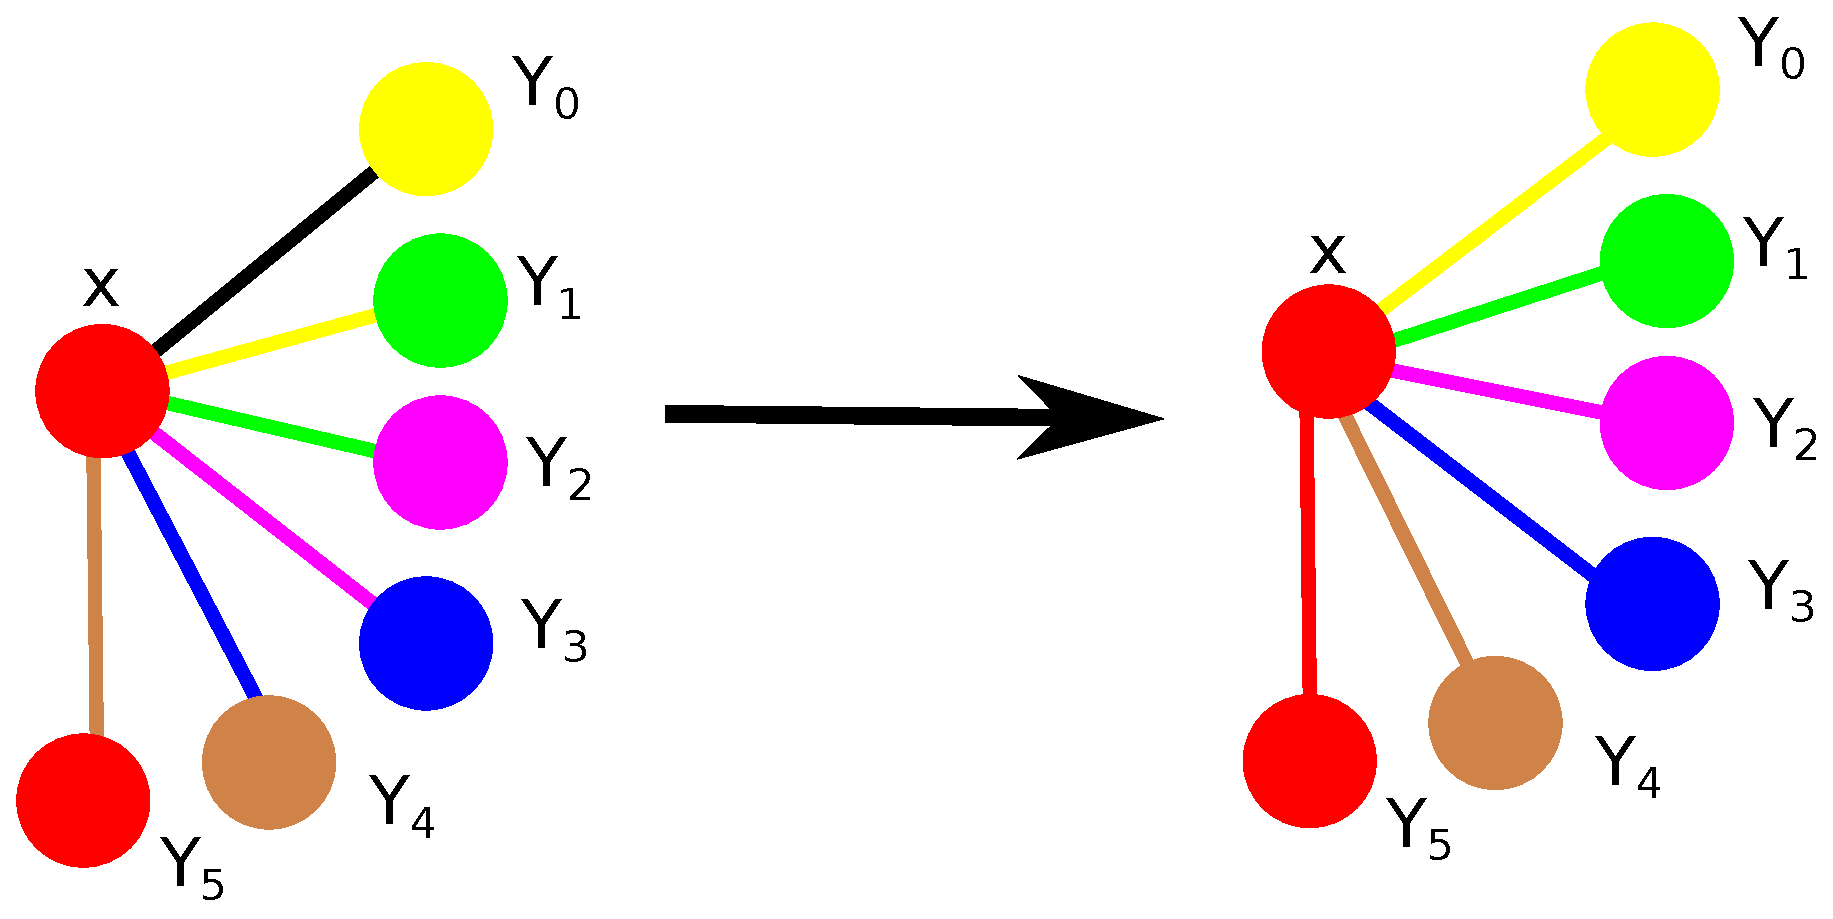
\includegraphics[width=0.40\textwidth]{pics/VIZING.eps}}}
	\caption{Důkaz Vizingovy věty. Barva vrcholu je volná barva u daného vrcholu. Chceme obarvit černou hranu.
			Případ kdy narazíme na vrchol jehož volná barva je stejná jako u x.
	} 
	\label{vizing_obr}
\end{figure}

\begin{figure}[h!]
	\centerline{\mbox{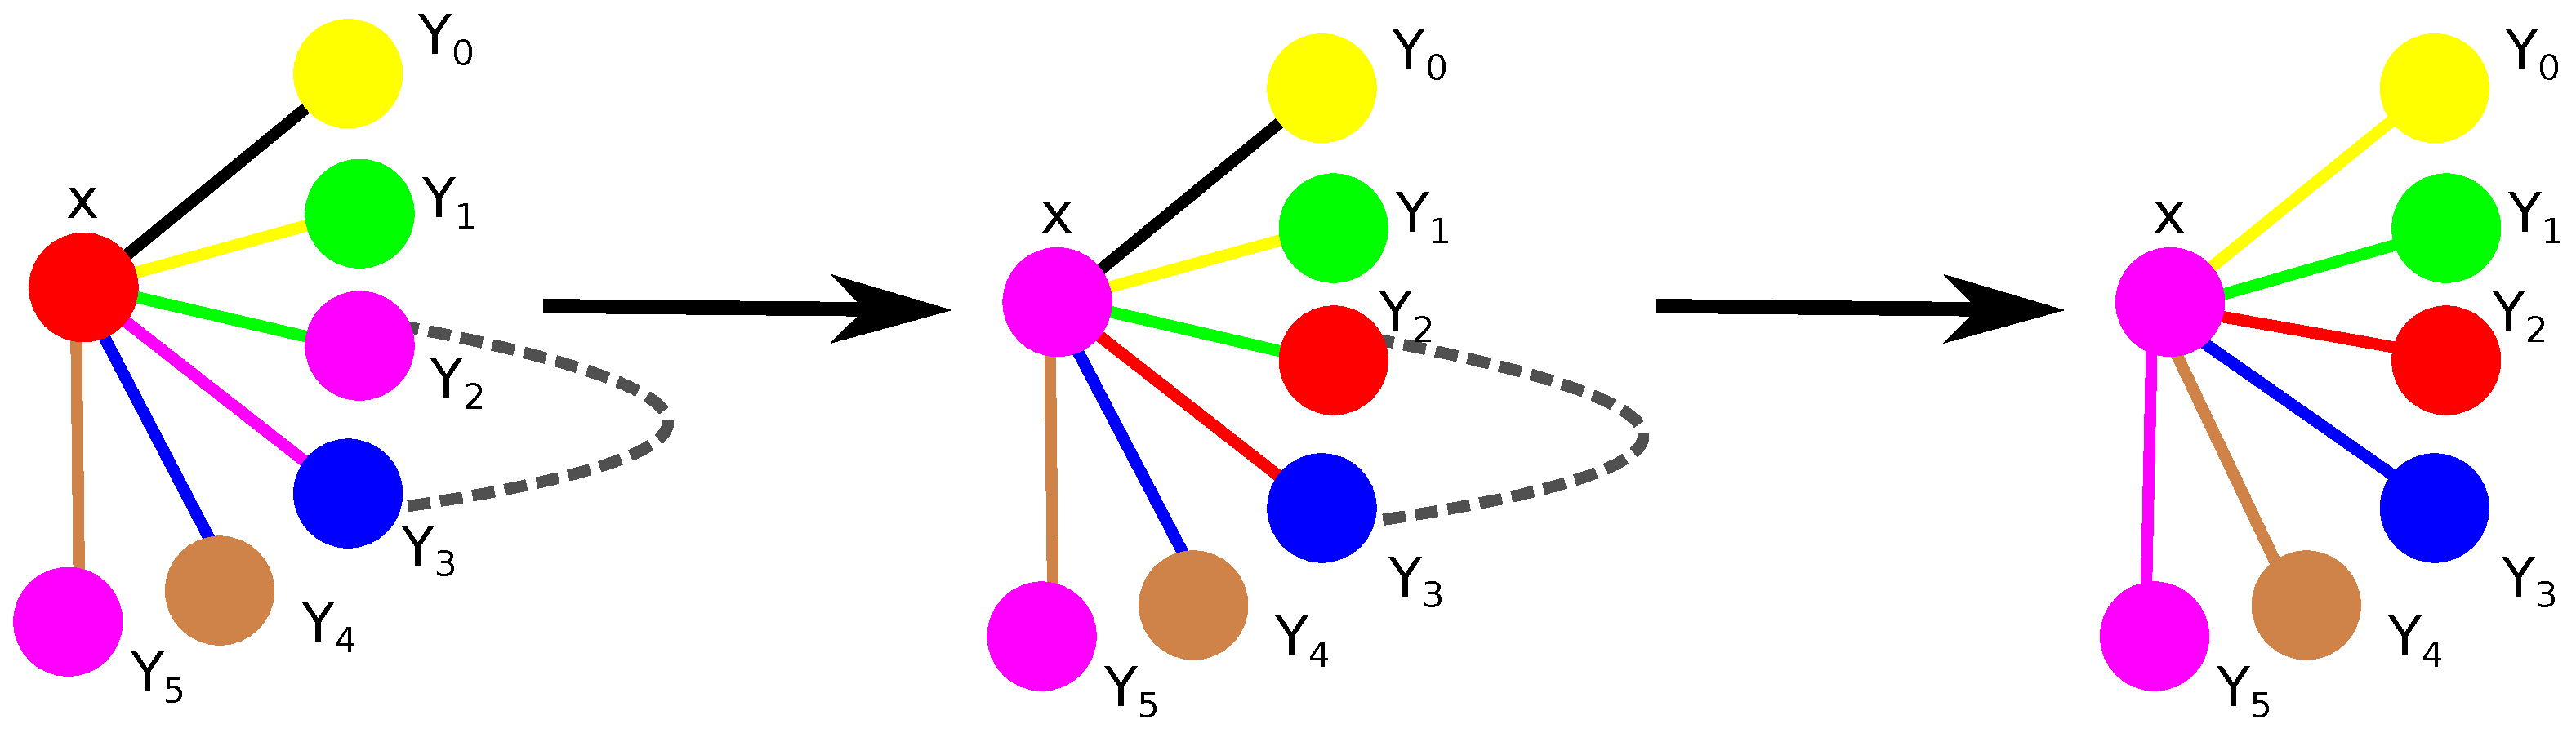
\includegraphics[width=0.80\textwidth]{pics/VIZING2.eps}}}
	\caption{Důkaz Vizingovy věty. Barva vrcholu je volná barva u daného vrcholu. Chceme obarvit černou hranu.
			Případ kdy narazíme na vrchol jehož volná barva je stejná jako u nějakého dřívějšího vrcholu $y_j$.
	} 
	\label{vizing_obr2}
\end{figure}

\medskip

\section{Tutteova věta}

\begin{define}
(Párování, Perfektní párování)

Párování v $G=(V,E)$ je množina hran $M \subset E$ taková, že každý vrchol je incidentní s nejvýše jednou hranou z $M$.

Perfektní párování (p.p.) je párování $M$ takové, že každý vrchol je incidentní s právě jednou hranou z $M$.
\end{define}

\begin{notation}
Počet lichých komponent grafu $G$ budeme značit $odd(G)$.
\end{notation}

Připomenutí Hallovy věty, dokazuje se např. pomocí toků v sítích.

\begin{theorem}
(Hallova věta)

Systém množin $S = {S_1, S_2, \ldots}$ má systém různých reprezentantů právě když pro každou $T \subset S$ platí:
\[
	\left|\bigcup_{M \in T}^{} M\right| \geq \left|T\right|.
\]
\end{theorem}


\begin{theorem}
(Tutteova věta)

Graf $G=(V,E)$ má perfektní párování $\Leftrightarrow \ \forall S \ |S| \geq odd(G\setminus S)$.
\end{theorem}

\begin{proof}
$\Rightarrow :$ V párování se spáruje vždy jeden vrchol každé z liché komponenty s jedním vrcholem z $S$.

$\Leftarrow :$ Dokazuje se sporem, nechť máme co nejmenší graf $G$ (co do počtu vrcholů), který podmínku nesplňuje.
Volíme co největší množinu $S$ tž. $|S| = odd(G\setminus S)$. Ukážeme:
\begin{enumerate}
\item $G\setminus S$ nemá sudou komponentu.
\item Každá lichá komponenta má perfektní párování po odebrání libovolného vrcholu.
\item Existuje párování $M_0$ tž. v každé liché komponentě je právě jeden vrchol incidentní s hranou v $M_0$.
\end{enumerate}

Pak z bodu $(3)$ vezmeme párování $M_0$, z bodu $(2)$ vytvoříme párování $M$ přídáním p.p. pro liché komponenty.
Z bodu $(1)$ plyne, že $M$ je p.p. v $G$.

$(1):$ Ze sudé komponenty zvolíme libovolný vrchol a přidáme ho do $S$ - spor s maximalitou $S$.

$(2):$ Nechť $C$ je lichá komponenta grafu $G$ v níž existuje $y$ tž. $C\setminus y$  nemá p.p.
Pak $C\setminus y$ nesplňuje Tutteovu podmínku (volili jsme nejmenší graf $G$).
\[
	\exists S'\ S' < odd(C\setminus S')
\]
\[
	|S\cup S' \cup y| - odd(G \setminus (S\cup S' \cup y)) \leq 1
\]
Spor s maximalitou $S$ protože pro včechna $T$ platí $|T| - odd(T)$ je sudé
($G$ má sudý počet vrcholů; $|V|=|T|+\sum_{C\ licha} |C| +\sum_{C\ suda} |C|$; přepočítáme modulo $2$).

$(3):$ Vyrobíme pomocný bipartitní graf (prohlásíme liché komponenty za vrcholy).
Ten splňuje Hallovu podmínku $\Rightarrow$ z Hallovy věty párování $M_0$.
Kdyby nesplňoval Hallovu podmínku $T_0$ (podmnožina vrcholů vzniklá z lichých komponent)
má sousedy $S_0$, kterých je méně než $|T_0|$. Pak graf $G$ nesplňuje Tutteovu podmínku pro $S_0$.
\end{proof}

\section{Extremální kombinatorika}

\subsection{Ramseyovy věty}

\begin{theorem}
(Ramseova věta - základní verze)

$\forall n \in \mathbb{N}$ $\exists N \in \mathbb{N}$, že graf na $N$ vrcholech obsahuje kliku velikosti $n$ nebo
nezávislou množinu velikosti $n$.

$\forall n_1, n_2 \in \mathbb{N}$ $\exists N \in \mathbb{N}$, že graf na $N$ vrcholech obsahuje kliku velikosti $n_1$ nebo
nezávislou množinu (NZMN) velikosti $n_2$.
\end{theorem}

\begin{proof}
Dokazujeme verzi s $n_1,n_2$ definujeme $R(n_1,n_2)$ jako minimální číslo, pro které tvrzení platí.

\[
	R(n_1,1) = R(1,n_2) = 1
\]
\[
	R(n_1,n_2) \leq R(n_1-1,n_2) + R(n_1,n_2-1)
\]
Protože vybereme jeden vrchol $v$ a vytvoříme množiny $A$ (vrcholy s hranou do $v$) a $B$ (vrcholy bez hrany do $v$).
Alespoň jedna má správnou velikost ($R(n_1-1,n_2)$ nebo $R(n_1-1,n_2)$) a z indukce má NZMN dané velikosti nebo o jedna menší.
Pokud má o jedna menší, přidáme $v$.
\end{proof}

\begin{theorem}
(Ramseova věta - vícebarevná verze)

$\forall n,b \in \mathbb{N}$ $\exists N \in \mathbb{N}$, že úplný graf na $N$ vrcholech jehož hrany jsou obarveny $b$ barvami
obsahuje jednobarevnou kliku velikosti alespoň $n$.
\end{theorem}

\begin{proof}
Indukcí dle počtu barev $b$, definujeme číslo $N(b,n)$ - nejmenší $N$ vzhledem k danému $n,b$, pro které věta platí.
Pro jednu a dvě barvy $N(1,n)=n$, $N(2,n)=R(n,n)$ - předchozí důkaz.
Pro větší počet barev $N(b,n) = R(N(b-1,n),n)$.
Z grafu na $N(b,n)$ vrcholech vybereme hrany jedné barvy a smažeme.
Z předchozí věty máme NZMN velikosti $n$ (jednobarevná klika velikosti n) nebo úplný graf velikosti $N(b-1,n)$.
Z indukce nalezneme jednobarevnou kliku velikosti $n$.
\end{proof}

\begin{theorem}
(Ramseova věta - nekonečná pro p-tice)

$\forall p,b \in \mathbb{N}$ $\forall f:\binom{\mathbb N}{p} \rightarrow B$ existuje nekonečná homogenní množina $X \subseteq \mathbb{N}$.
\end{theorem}

\begin{proof}
Indukcí dle $p$, pro $p=1$ jednoduché.
Tvoříme posloupnost nekonečných množin $A_0 = \mathbb{N},A_1, \ldots $.
Z $A_i$ si vybereme si libovolný prvek $v_i$ ten odstraníme a vytvoříme funkci $f'$ obarví $(p-1)$-tici $Q$ barvou $f(Q+v_i)$
(barvou původní $p$-tice obsahující $v_i$).
Dle indukce existuje nekonečná homogenní podmnožina pro $f'$ tu zvolíme jako $A_{i+1}$.
Opakujeme až dostaneme nekonečnou posloupnost prvků $v_0,v_1, \ldots $.
 
Z konstrukce je barva hrany $(v_i, v_j)$ pro $i<j$ je závislá jen na $v_i$.
Obarvíme si prvek $v_i$ barvou, kterou mají hrany $v_i,v_j$ pro $i<j$.
Barev je konečně mnoho, z principu holubníku se nějaká opakuje nekonečně krát.
Nechť její výskyty $v_{g(1)},v_{g(2)}, \ldots$ pak prvky $v_{g(1)},v_{g(2)}, \ldots$
tvoří nekonečnou homogenní podmnožinu $\mathbb{N}$.
\end{proof}

\subsection{Erd\H{o}s-Ko-Radoova věta}

\begin{define}
($k$-uniformní hypergraf)

$k$-uniformní hypergraf je dvojice množin $(V,E)$ kde $E$ je množina $k$-prvkových podmnožin $V$.
\end{define}

\begin{notation}
$f_k(n)$ značí největší počet hran $k$ uniformního hypergrafu takový, že každé dvě hrany mají neprázdný společný průnik.
\end{notation}

\begin{theorem}
(Erd\H{o}s-Ko-Radoova věta)

Pro $n\geq 2k$: $f_k(n) = \binom{n-1}{k-1}$.
\end{theorem}

TODO: tenhle důkaz doprojít dovysvětlit..

\begin{proof}
$\geq :$ volíme různé hrany, kde všechny obsahují jeden vybraný vrchol.

$\leq :$ "Interval" označíme množinu $\{i,i+1,\ldots i+k-1\}$ pak $E$ obsahuje maximálně $k$ intervalů.
(BÚNO: $E$ obsahuje interval $\{1,2,\ldots k\}$, navíc $E$ obsahuje vždy maximálně jeden z intervalů 
$\{i,i+1,i+2,\ldots i+k-1\}$ a $\{i-1,i-2,\ldots i-k\}$.)

Počítáme dvěma způsoby dvojice $(\sigma,e)$ kde $e$ je hrana a $\sigma(e)$ je interval:
\begin{enumerate}
\item počet dvojic $\leq n! \cdot k$ (máme $n!$ permutací, každá má nejvýše $k$ intervalů v $|E|$)
\item $|E| \cdot n \cdot k! \cdot (n-k)! = $ počet dvojic
	(vybereme náhodnou hyperhranu a máme $n \cdot k! \cdot (n-k)!$ (výběr prvního prvku krát permutace prvků intervalu krát
	premutace ostatních prvků) zobrazení $k$-prvkové množiny na interval)
\end{enumerate}
Pak dostáváme 
\[
	|E| \leq \frac{n! \cdot k}{ n \cdot k! \cdot (n-k)!} = \frac{k}{n}\binom{n}{k} = \binom{n-1}{k-1}.
\]
\end{proof}

\medskip

\section{Samoopravné kódy}

Máme kód nad $\mathbb{Z}_2$.

\begin{example}
Trojitý opakovací kód $0 \rightarrow 000$ a $1 \rightarrow 111$
Kontrola parity $(x_1,x_2,x_3) \in \mathbb{Z}_2^3 \rightarrow (x_1,x_2,x_3,x_1+x_2+x_3)$
\end{example}

\begin{define}
Hemingova váha slova - počet jedniček, které obsahuje

Hemingova vzdálenost slov - počet pozic, ve kterých se daná slova liší
\end{define}

TODO chybí samoopravné kódy
\medskip

\section{Pravděpodobnostní metoda - příklady použití}

Nekonstruktivní metoda dokazů používaná v kombinatorice.
Dokazuje se existence objektu s danými vlastnostmi.
Vezmeme náhodný objekt a dokážeme, že pravděpodobnost, že nemá danou vlastnost je menší než $1$.
Potom existuje objekt s danou vlastností.


Příklad použití pravděpodobnostní metody
\begin{theorem}
Mějme množiny $S_1, S_2, \ldots S_m$, kde $|S_i| = l$
Pak je-li $m < 2^{l-1}$ můžeme obarvit $\bigcup_{1\leq i \leq m} S_i$ dvěmi barvami tak, že žádná $S_i$ není monochromatická.
\end{theorem}

\begin{proof}
Každému prvku náhodně nezávisle přiřadíme barvu.
$B_{S_i}$ označíme jev, že množina $S_i$ je monochromatická, pak:
\[
	P[B_{S_i}] = \frac{1}{2^l} + \frac{1}{2^l} = \frac{1}{2^{l-1}}.
\]
Pravděpodobnost, že je libovolná množina monochromatická je 
\[
	\sum_i P[B_{S_i}] = m \cdot \frac{1}{2^{l-1}} < 1.
\]
\end{proof}

TODO: nějaký další hezký jednoduchý příklad

\end{document}

